
\begin{figure*}[hbt!]
\centering
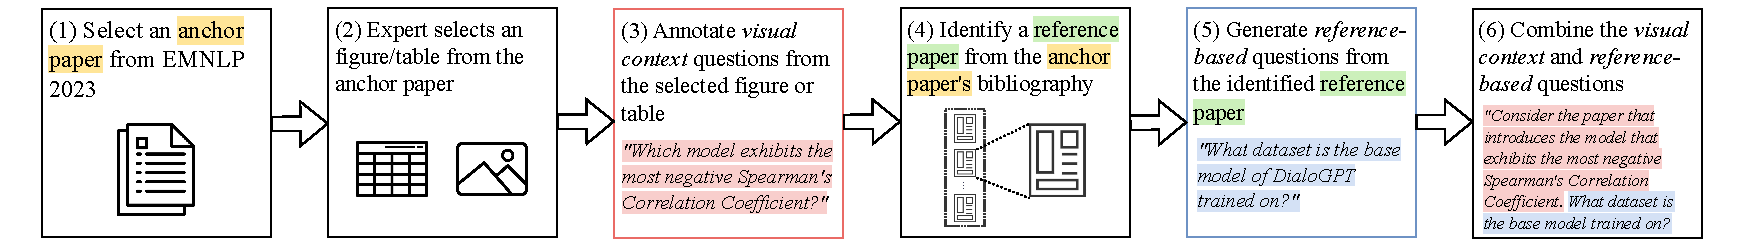
\includegraphics[width=1\textwidth]{raw_figures/construction_pipeline.pdf}
\caption{
An overview of \data question construction pipeline.
}
\label{fig:pipeline}
\end{figure*}
\section{The \data Benchmark} 
\subsection{Overview of \data}
\label{sec:overview}


Our objective is to develop a challenging yet realistic QA benchmark that necessitates both \emph{multi-modal} and \emph{multi-document} reasoning over scientific papers. 
%to meet the requiremtns/ to fulfill the goal, we define 2 intermediate xxx 
%
% \ziyao{a bit confusing; maybe no need to explain here; the benchmark itself mainly features the combined question; it sounds untrue to directly claim the benchmark contains two types of questions because as we clarified in the rebuttal their existences are in fact a compromise during evaluation}
%
To achieve this objective, we define two types of intermediate questions in our question construction pipline: 
%
% 
\vspace{-0.2em}
\begin{itemize}[leftmargin=*]
    \itemsep0em 
    \item \textbf{Visual Context Question}: A question derived from a figure or table of an \textit{anchor paper}, with its answer pointing to a \textit{reference paper}. Each figure or table can correspond to multiple visual context questions.
    %
    \item \textbf{Reference-based Question}: A question regarding a specific detail in the \textit{reference paper}. Each visual context question can correspond to multiple reference-based questions. 
\end{itemize}
%
The final \textit{combined questions} are created by combining each visual context question with each of its related reference-based questions.
%
The overview of this pipeline is shown in Figure \ref{fig:pipeline}. 
%
In constructing \data, expert annotators are tasked with composing visual context questions from the 70 curated anchor papers, adhering to four pre-defined reasoning categories: \emph{comparisons}, \emph{data extraction}, \emph{locations}, and \emph{visual understanding} (Table \ref{tab:locality_reasoning} in Appendix~\ref{app:locality_reasoning_examples}).
%
By answering a visual context question, expert annotators can pinpoint a reference paper that provides further elaboration on the topic from among all the publications cited by the anchor paper. 
%
Subsequently, GPT-4\footnote{\texttt{gpt-4-0125-preview}}
is employed to generate reference-based questions from the identified reference paper. 
%
GPT-4 is utilized again to rephrase and combine each visual context question with each of the related reference-based questions to form a comprehensive question that embodies both multi-modal and multi-document reasoning.
%
Finally, expert annotators are tasked with verifying the quality of these GPT-4-assisted questions.
% 
Statistics of the benchmark are listed in Table \ref{tab:dataset_statistics}; 
%
distributions of reasoning types across visual context and reference-based questions are illustrated in Figure \ref{fig:reasoning_distribution}.



\begin{figure*}[!ht]
    \centering
    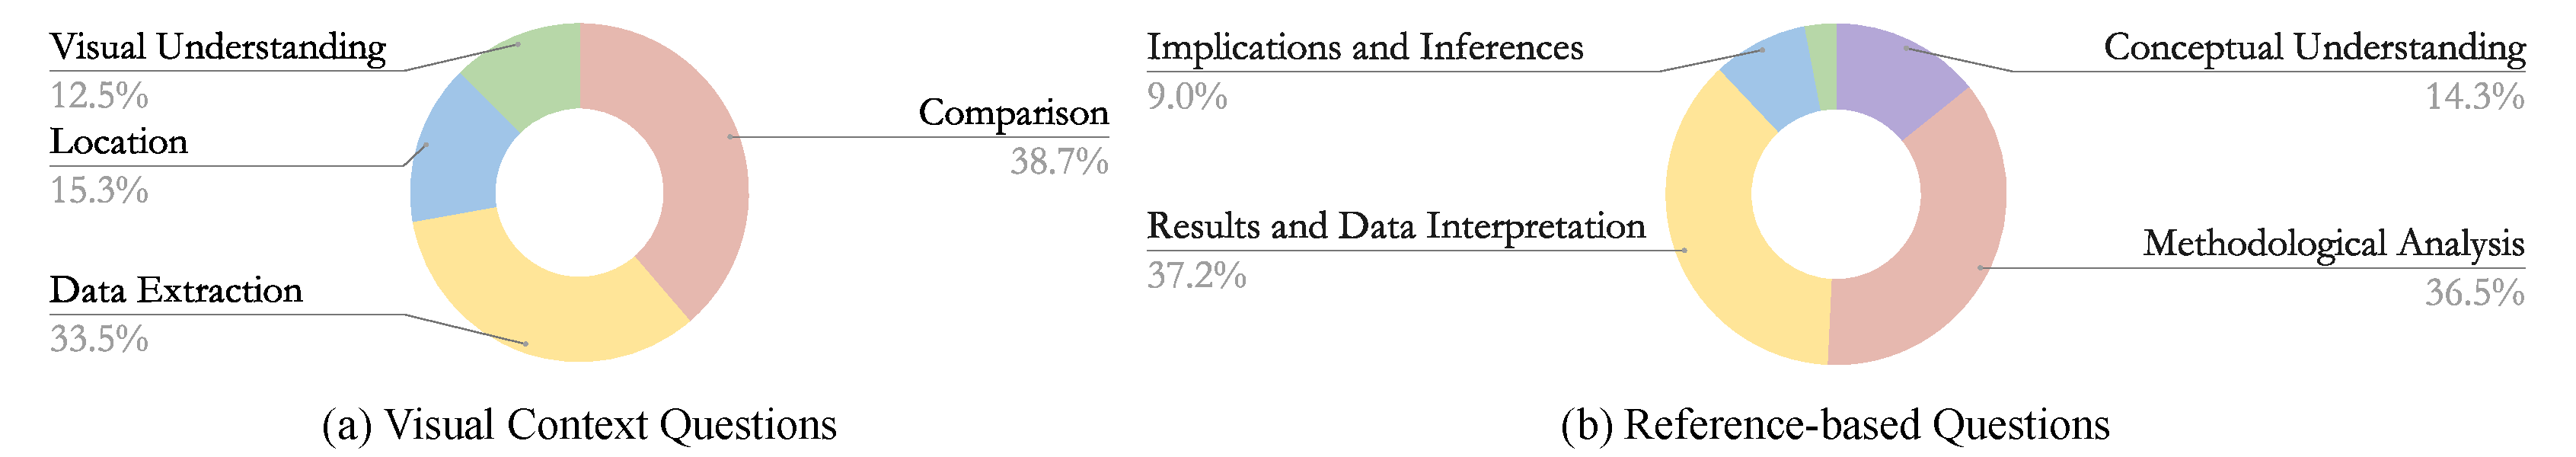
\includegraphics[width=\textwidth]{raw_figures/reasoning_distribution.pdf}
    \caption{Distribution of reasoning types of \emph{visual context} and \emph{reference-based} questions in \data.} 
    \label{fig:reasoning_distribution}
\end{figure*}
\subsection{Benchmark Construction Principles}


To bridge the gap in current benchmarks that separately assess either multi-modal or multi-document reasoning, our benchmark, \data, aims to encompass both elements in a single QA pair. 
%
Therefore, our benchmark construction pipeline adheres to the following guidelines:
%
(1) it includes diverse modalities, such as texts, figures (including line plots, bar plots, scatter plots, etc.), and tables (stored as images to preserve format integrity rather than as plain texts); 
%
(2) it necessitates connecting information across multiple documents; 
%
(3) it spans a variety of reasoning types, including four types of visual context reasoning and five types of reference-based reasoning;
%
(4) it poses significant challenges in both \emph{multi-modal} comprehension and \emph{multi-document} information retrieval; and 
%
(5) it generates realistic QA pairs that reflect the workflows common in scientific literature analysis.


\subsection{Benchmark Construction}
\label{sec:benchmark_construction}

\paragraph{Expert Annotators.}
We recruit three computer science graduate students with expertise in the field of NLP, each of whom have authored at least one peer-reviewed publication in top-tier NLP conferences. 
%
Their responsibilities include: 
%
(1) curating anchor papers from a pool of candidates and composing visual context questions; 
%
(2) reviewing and verifying the reasoning types of reference-based questions; 
%
(3) resolving discrepancies between answers generated from the two rounds of reference-based answer generation; 
%
and (4) checking consistency, clarity, and redundancy in the combined questions. 
%
Further details on annotations are provided in Appendix \ref{sec:expert_annotation_details}.

\paragraph{Anchor Papers.} 
%
To mitigate the risk of data contamination, where models might rely on pre-trained knowledge to answer the visual context questions rather than analyzing the provided scientific images, we curate anchor papers from a recent NLP conference, EMNLP 2023. 
%
Among the 1,047 papers accepted by EMNLP 2023, we select 441 papers that were released on arXiv after October 1st, 2023 as candidate anchor papers. 

\paragraph{Visual Context QAs from Anchor Papers.} 
%
Two of the expert annotators curate 70 papers by manually examining 441 candidate anchor papers collected. Subsequently, they select 21 figures and 62 tables from the 70 papers to compose 300 visual context questions and answers that conform to four visual reasoning types.
%
The ground truth answer to each visual context question is the single reference paper to which the visual context question directly refers.
%
This facilitates a transition from an anchor paper to a reference paper that elaborates on the subject.
%
The third annotator is responsible for validating the accuracy and relevance of these questions and answers.
%
371 papers are excluded in this process because they either lack figures or tables that can be analyzed by one of the reasoning types, or transition to a cited paper that is not available on arXiv.
%
Furthermore, due to the occurrence of identical answers among some visual context questions, these 300 questions correspond to only 107 reference papers.




\paragraph{Reference-Based QAs from Reference Papers.} 
By requiring that the 107 reference papers be available on arXiv, we ensure access to their complete content.
%
This enables us to utilize GPT-4 to generate open-ended, reference-based questions from the papers.
%
For each reference paper, we create five questions each corresponding to a reasoning type illustrated in Table \ref{tab:detail_reasoning_definition} in \ref{app:detail_reasoning_def}. 
%
These questions are designed to be answerable in a text-only setting, without the need for visual reasoning or OCR. 
%
Considering the possibility that GPT-4 may incorrectly categorize the questions, expert annotators manually examine the reasoning types associated with the questions and reassign when necessary. 
%
This process yields a total of 519 reference-based questions after filtering out duplicates, overly complex questions, questions that do not require specific insights from the paper (\eg ``What is the mathematical expression for calculating the F-1 score?''), and questions that do not belong to any of the five predefined reasoning types.
To establish a \emph{gold answer} for each question, we generate answers in two rounds. 
%
In the first round, answers are generated concurrently with the questions. 
%
In the second round, the model is prompted to answer the questions using the reference paper as context. 
%
We employ GPT-4 to determine whether the answers from both rounds are consistent. 
%
If any discrepancy is identified, expert annotators are enlisted to verify and finalize the answers. 
%
Further details can be found in Appendix \ref{2_round_checking}.


\paragraph{Combined Questions.} 
%
We utilize GPT-4 to compile the final questions for the benchmark by combining each visual context question with its corresponding reference-based questions. 
%
After the combination, expert annotators are tasked with verifying the question validity and rephrasing the GPT-4-assisted combined question when necessary.
%
Overall, we form \datanum combined questions, each associated with a specific figure or table. 
%
Expert annotators then review these combined questions to ensure that each visual context question and its corresponding reference-based questions are logically connected and relevant. 
%
They also check for clarity, consistency, and redundancy to maintain the quality and difficulty of the benchmark.


\begin{table}[!t]
\centering
\small
    \begin{tabular}{lr}
        \toprule
        \bb{Statistics} & \bb{\emph{Avg.} Value}   \\ 
        \midrule
        Visual Context Question Length \emph{(tokens)} & 12.9 \\
        Reference-based Question Length \emph{(tokens)} & 25.95 \\
        Combined Question Length \emph{(tokens)}  & 41.3 \\
        Answer Length \emph{(tokens)} & 24.9\\
        \addlinespace[0.2em]\hdashline\addlinespace[0.2em]
        \# Cluster & 70 \\
        \# Anchor Paper per Cluster & 1 \\
        \# Reference Paper per Cluster & 42.8\\
        Paper Length \emph{(tokens)} & 11.8K \\
        \midrule
        Validation Set Size  & 452 \\
        Test Set Size & 1000 \\
    
        \bottomrule
    \end{tabular}
    \caption{Key statistics of the \data benchmark.}
    \label{tab:dataset_statistics}
\end{table}

